% !TEX encoding = UTF-8
% !TEX TS-program = pdflatex
% !TEX root = ../tesi.tex

%**************************************************************
\chapter{Progettazione}
\label{cap:progettazione}
%**************************************************************

In questo capitolo verrà descritta la progettazione dell'intero prodotto, in particolare verranno chiariti i seguenti argomenti:
\begin{itemize}
	\item progettazione delle classi che definiscono lo stato dell'applicazione;
	\item gestione dello stato dell'applicazione;
	\item progettazione del parser Json e dell'\emph{adapter} per trasformare le informazioni ottenute dall'api nelle classi che definiscono lo stato dell'applicazione;
	\item gestione del caricamento parziale dei dati della tabella;
	\item descrizione e progettazione dei componenti grafici.
\end{itemize}

\section{Entità dello stato}
Per quanto riguarda lo stato dell'applicazione ho analizzato la struttura e le funzionalità della tabella fornita dall'azienda. Durante la progettazione della struttura dello stato ho dato priorità alla semplicità in modo da avere funzioni di renderizzazione concise e facili da manutenere. Dalla struttura della tabella pivot e dalla descrizione delle sue funzionalità ho ricavato le seguenti strutture dati:

\paragraph*{data class DimensionsNode}- rappresenta una cella d'intestazione, deve contenere:
\begin{itemize}
	\item \verb|id|: codice della cella;
	\item \verb|label|: testo da renderizzare;
	\item \verb|level|: indica a che dimensione dell'intestazione appartiene la cella;
	\item \verb|childDepth|: indica la profondità della cella in una gerarchia ad albero;
	\item \verb|path|: codice identificativo della cella costituito da una lista di \verb|id| che rappresenta la gerarchia di una cella;
	\item \verb|actionType|: indica il tipo dell'azione che bisogna eseguire, esso verrà indicato con una classe di tipo: \verb|enum class NodeActionType|;
	\item \verb|isChild|: indica se la cella è un figlio di un'altra cella.
\end{itemize}

\paragraph*{data class BodyCells}- rappresenta una cella dei dati, deve contenere:
\begin{itemize}
	\item \verb|value|: indica il dato;
	\item \verb|cPath|: indica l'insieme dei codici delle dimensioni delle colonne a cui appartiene il dato;
	\item \verb|rPath|: indica l'insieme dei codici delle dimensioni delle righe a cui appartiene il dato.
\end{itemize}	

\paragraph*{data class HeaderAction}- rappresenta una azione sulle dimensioni, deve contenere:
\begin{itemize}
	\item \verb|actionType|: indica il tipo dell'azione che bisogna eseguire, esso verrà indicato con una classe di tipo: \verb|enum class NodeActionType|;
	\item \verb|dim|: indica la dimensione su cui applicare l'azione;
	\item \verb|depth|: indica la profondità all'interno della dimensione su cui applicare l'azione.
\end{itemize}

\paragraph*{enum class NodeActionType}- rappresenta un tipo di azione che può essere:
\begin{itemize}
	\item \verb|EXPAND|: indica che la cella può espandere per mostrare i suoi figli;
	\item \verb|COLLAPSE|: indica che la cella può nascondere i suoi figli;
	\item \verb|NULL|: indica che la cella non ha un'azione.
\end{itemize}
\noindent
Quindi per rappresentare l'intero stato della tabella ho definito un ultimo \verb|data class|:
\paragraph*{data class TableState}
\begin{itemize}
	\item \verb|rows|: matrice di DimensionsNode, rappresenta le dimensioni delle righe;
	\item \verb|cols|: matrice di DimensionsNode, rappresenta le dimensioni delle colonne;
	\item \verb|cells|: matrice di BodyCells, rappresenta le celle contente i dati della tabella;
	\item \verb|rowActions|: matrice di HeaderAction, rappresenta le azioni disponibili per le dimensioni delle righe;
	\item \verb|colActions|: matrice di HeaderAction, rappresenta le azioni disponibili per le dimensioni delle colonne.
\end{itemize}

\section{Gestione dello stato}
In questa sezione verrà descritto il ragionamento e il modo in cui è avvenuta la progettazione degli elementi che si occuperanno di gestire lo stato dell'applicazione.

\subsection{Dataflow dell'applicazione}
Un aspetto che è stato molto discusso dal team di sviluppo riguarda il \gls{dataflowg} dell'applicazione. Durante la prima settimana del tirocinio, oltre allo studio delle tecnologie, si è pensato a come verrà gestito lo stato dell'applicazione e in particolare alle possibili soluzioni per garantirne la scalabilità. Nelle prossime sezioni verranno descritti i \emph{dataflow} forniti da React e Redux, infine verrà identificato quello adottato nell'ambito del progetto.

\subsubsection*{React}
React è una libreria per realizzare interfacce utente che utilizza un \emph{dataflow} unidirezionale, questo significa che il flusso dei dati deve passare mediante dei componenti grafici. I dati possono essere contenuti nello stato locale di un componente che è accessibile solo dal componente stesso. Le informazioni possono invece essere passate tra un componente padre ai suoi componenti figli mediante le \gls{propsg}. \\
Questo \emph{dataflow} è molto semplice da utilizzare però presenta alcune limitazioni per quanto riguarda la scalabilità. Per avere uno stato unico di tutta l'applicazione bisognerebbe dare ad un componente grafico la responsabilità di mantenerlo nel suo stato locale. L'architettura che ne deriva, nel caso di applicazioni complesse, è difficile da manutenere e poco scalabile. \\
Tuttavia questo semplice \emph{dataflow} ha il vantaggio che per un numero ristretto di componenti i cambiamenti di stato locale e i passaggi di informazioni mediante le \emph{props} sono molto veloci e semplici.

\subsubsection*{Redux}
Per garantire scalabilità nella gestione dello stato dell'applicazione è stato deciso di utilizzare la libreria Redux. Essa offre un \emph{dataflow} unidirezionale dove lo stato è gestito all'intero di una una struttura di Redux chiamata \emph{store}. Questa struttura è esterna ai componenti grafici, quindi la gestione dello stato dell'applicazione diventa prevedibile e manutenibile. Redux si basa su tre principi:
\begin{itemize}
	\item lo stato è l'unica fonte di verità;
	\item lo stato non è modificabile direttamente;
	\item le modifiche avvengono medianti \gls{purefunctionsg} che creano un nuovo stato per evitare \emph{side effects} .
\end{itemize}

\noindent
Gli elementi dell'architettura di Redux sono i seguenti:
\begin{itemize}
	\item \textbf{Actions}: oggetti che rappresentano un'azione che innesca un cambiamento dello stato;
	\item \textbf{Reducers}: \emph{funzioni pure} che accettano come parametro un \emph{actions} e si occupano di modificare lo stato generandone una copia modificata;
	\item \textbf{Store}: lo \emph{store} è un'interfaccia che contiene lo stato dell'applicazione e fornisce funzioni per leggere, modificare e registrare \emph{listeners}\glosp allo stato.
\end{itemize}

\subsection{Soluzione}
Per lo sviluppo di questo componente oltre all'architettura Redux descritta nella sezione precedente è stato utilizzato anche il \emph{dataflow} di React per gestire gli aggiornamenti visivi. Il \emph{dataflow} finale del prodotto è quindi il seguente:
\begin{enumerate}
	\item se l'utente esegue un'azione che implica un cambiamento dello stato verrà mandata allo \emph{store} un \emph{actions};
	\item lo \emph{store} si occuperà di chiamare un \emph{reducer} in modo da ricevere lo stato successivo;
	\item lo stato verrà aggiornato e i cambiamenti saranno visibili a tutti i componenti React che sono registrati allo Store.
\end{enumerate}
Per applicare al meglio il \emph{dataflow} precedentemente descritto ho progettato i componenti di Redux nel seguente modo. Per prima cosa ho suddiviso lo stato dell'applicazione in \emph{slice} cioè in sezioni di stato. In questo modo la sua struttura è modulare e scalabile dato che, se questa applicazione verrà ampliata basterà aggiungere uno \emph{slice} allo stato. Ogni slice deve essere definito nel seguente modo:
\begin{lstlisting}[caption={Esempio Slice}, label={lst:slice_state}, language=Kotlin]
object Slice {
	// Stato
	data class State( ... )
	
	// Thunk
	private val thunk = Thunk()
	fun funcThunk() : RThunk = thunk
	
	// Actions
	class Action(): RAction
	...
	
	// Reducer
	fun reducer(state: State = State(), action: RAction) : State { ... }
}
\end{lstlisting}

\subsubsection*{Stato}
In ogni \emph{slice} deve essere definito un \verb|data class| che contiene tutti i campi dati che definiscono lo stato. Per quanto riguarda la realizzazione della tabella pivot ho individuato la necessità di uno \emph{slice} con i seguenti campi dati:
\begin{itemize}
	\item \verb|isLoading|: valore booleano che indica se si stanno effettuando chiamate http o funzionalità asincrone;
	\item \verb|rows|: insieme di celle che rappresentano le dimensioni delle righe;
	\item \verb|cols|: insieme di celle che rappresentano le dimensioni delle colonne;
	\item \verb|cells|: insieme di celle che contengono i dati relativi alle dimensioni;
	\item \verb|rowTree|: struttura ad albero che definisce la relazione tra le dimensioni delle righe;
	\item \verb|colTree|: struttura ad albero che definisce la relazione tra le dimensioni delle colonne;
	\item \verb|rowActions|: insieme di possibili azioni eseguibili sulle dimensioni delle righe;
	\item \verb|colActions|: insieme di possibili azioni eseguibili sulle dimensioni delle colonne.
\end{itemize}

\subsubsection*{Actions}
Le actions sono definiti come delle classi di tipo \verb|RAction| che vengono usati per innescare l'update dello stato. Solitamente un'\emph{action} si occuperà di modificare solo un campo dato dello stato. Quindi dalla mia precedente progettazione dello stato ho individuato cinque \emph{actions}:
\begin{itemize}
	\item \verb|class SetIsLoading(): RAction|;
	\item \verb|class UpdateRows(): RAction|;
	\item \verb|class UpdateCols(): RAction|;
	\item \verb|class UpdateCells(): RAction|;
	\item \verb|class UpdateRowTree(): RAction|;
	\item \verb|class UpdateColTree(): RAction|;
	\item \verb|class UpdateRowActions(): RAction|;
	\item \verb|class UpdateColActions(): RAction|.
\end{itemize}

\subsubsection*{Thunk}
Nell'ambito di questo progetto i cambiamenti dello stato devono essere gestiti in modo asincrono, in quanto viene fornita una \emph{API} di supporto. Dato che i cambiamenti allo stato innescati dalle \emph{actions} possono essere solo sincroni ho utilizzato un \emph{middleware} di Redux che fornisce le stesse funzionalità di un \emph{actions} ma ne espande l'utilità permettendo operazioni asincrone, questa interfaccia è definita come \verb|thunk|.
I \emph{thunk} sono usati per effettuare operazioni asincrone complesse, l'interfaccia dei \emph{thunk} purtroppo non era presente nell'implementazione di Redux di kotlin quindi ho realizzato una semplice interfaccia che ne implementa le sue funzionalità più significative. In particolare l'esecuzione asincrona degli update dello stato.
\begin{lstlisting}[caption={Interfaccia Thunk}, label={lst:thunk_interface}, language=Kotlin]
interface RThunk : RAction {
	operator fun invoke(
	dispatch: (RAction) -> WrapperAction,
	getState: () -> AppState
	) : WrapperAction
}

fun rThunk() =
applyMiddleware<AppState, RAction, WrapperAction, RAction, WrapperAction>(
{ store ->
	{ next ->
		{ action ->
			if (action is RThunk)
			  action(store::dispatch, store::getState)
			else
			  next(action)
		}
	}
}
)

val nullAction = js {}.unsafeCast<WrapperAction>()
\end{lstlisting}

\subsubsection*{Reducer}
Un \emph{reducer} è una \emph{funzione pura} che riceve come argomento un \verb|RAction| e ritorna una copia dello stato modificato. In kotlin il modo per realizzare una funzione \emph{reducer} è utilizzare una struttura \emph{switch} (in kotlin corrisponde ad una struttura \emph{when}) dove vengono definiti tanti casi quanto sono le \emph{actions} disponibili che vogliono essere utilizzate. Per le \emph{actions} definite precedentemente:
\begin{lstlisting}[caption={Interfaccia Thunk}, label={lst:reducer_slice}, language=Kotlin]
fun reducer(state: State = State(), action: RAction) : State {
  return when (action) {
    is SetIsLoading -> state.copy(...)
    is UpdateRows -> state.copy(...)
    is UpdateCols -> state.copy(...)
    is UpdateRowTree -> state.copy(...)
    is UpdateColTree -> state.copy(...) 
    is UpdateCells -> state.copy(...)
    is UpdateRowActions -> state.copy(...)
    is UpdateColActions -> state.copy(...)
    else -> state
  }
}
\end{lstlisting}


\section{Parser e adapter}
Per quanto riguarda la progettazione del parser Json per l'api ho per prima cosa definito i passaggi necessari per ottenere i dati dall'API di Gruppo4. Ho individuato la necessità di due funzioni \verb|fetch| e \verb|sendAction|, la prima per richiedere i dati iniziali e la seconda per ottenere nuovi dati in seguito ad un'azione effettuata da un utente. \\
Per realizzare il parser ho studiato la struttura del Json ritornato dall'API in modo da identificare tutte le data class \verb|@Serializable| che mi permetteranno di mappare il Json in \verb|data class|. La struttura del Json è la seguente:
\begin{lstlisting}[caption={Struttura JSON API}, label={lst:json_structure}, language=json]
{
	"Rows": {
		"Paths": [
		["_all", "_all", ...], [ ... ]
		],
		"Actions": [
		{ "Action": "C", "Dim": 1, "Depth": 0 }, { ... }
		],
		"Tree": [
		{
			"Code": "_all",
			"Label": "All",
			"SubDim": [
			{
				"Code": "_all",
				"Label": "All",
				"SubDim": null,
				"Children": null
			}
			]  
		}
		]
	}
	"Cols": // stessa struttura di "Rows"
	"Cells": [
	  [51515, 2315, 747, 22],
	  [ ... ]
	],
	"Filters": [
	  {
	    "Filtered": false,
	    "ActiveFilters": ["f1", "f2", "f3"],
	    "Type": "list",
	    "Name": "associazioni_provincia",
	    "Label": "Associazioni per provincia"
	  }
	]
}
\end{lstlisting}
Da questa struttura ho identificato le seguenti \verb|data class @Serializable|:
\begin{itemize}
	\item \verb|Gruppo4Json|: rappresenta la struttura generale del Json;
	\item \verb|Gruppo4Data|: rappresenta la struttura dei campi dati "Rows" e "Cols";
	\item \verb|Gruppo4Filter|: rappresenta la struttura contenuta nel campo dati "Filters";
	\item \verb|Gruppo4Actions|: rappresenta la struttura contenuta nel campo dati "Actions" all'interno di "Rows" e "Cols";
	\item \verb|Gruppo4Node|: rappresenta la struttura contenuta nel campo dati "Tree" all'interno di "Rows" e "Cols" e corrisponde ad un nodo della struttura ad albero.
\end{itemize}
\noindent
Per quanto riguarda la progettazione dell'adapter ho analizzato le data class ottenibili dal Json e le \verb|data class| definite nello stato. Da questa analisi ho individuato le seguenti funzioni da realizzare:
\begin{itemize}
	\item \verb|fun convertListOfGruppo4Node()|:
	\begin{itemize}
		\item si occuperà di convertire una lista di \verb|Gruppo4Node| in \verb|DimensionsNode|;
	\end{itemize}

	\item \verb|fun convertTree()|:
	\begin{itemize}
		\item si occuperà di convertire la struttura ad albero in una struttura più semplice da iterare;
	\end{itemize}
	
	\item \verb|fun convertListOfGruppo4Actions()|:
	\begin{itemize}
		\item si occuperà di convertire una lista di \verb|Gruppo4Actions| in \verb|HeaderAction|;
	\end{itemize}

	\item \verb|fun convertCells()|:
	\begin{itemize}
		\item si occuperà di unire i dati definiti nel campo dati "Cells" con i "Path" in modo da ottenere una matrice di \verb|BodyCells|.
	\end{itemize}
\end{itemize}

\section{Gestione del caricamento parziale}
L'azienda ha identificato due requisiti riguardanti il caricamento parziale dei dati della tabella in modo da non sovraccaricare l'\emph{API} con file Json troppo grandi. In particolare mi ha richiesto di implementarlo sotto due aspetti. Il primo riguarda il caricamento parziale di informazioni quando si "apre" una cella d'intestazione delle dimensioni. Il secondo invece riguarda il caricamento parziale durante lo scroll di un utente.

\subsection*{Caricamento parziale di un nodo}
Le dimensioni di analisi della tabella pivot vengono fornite dall'\emph{API} sotto forma di struttura ad albero, da cui verrà generata una matrice di oggetti in modo da semplificare l'iterazione di essa all'interno della funzione \verb|render()| dei componenti React. La struttura ad albero fornisce però dei vantaggi per quanto riguarda il caricamento parziale di un nodo infatti basterà modificare un nodo dell'albero e poi generare la matrice di oggetti. Per farlo ho pensato di mantenere nello stato una copia della struttura ad albero, in questo modo quando viene aperto o chiuso una cella di una dimensione della tabella basterà semplicemente sostituire il nodo nella copia della struttura ad albero dello stato e generare nuovamente la matrice di oggetti.

\subsection*{Caricamento parziale scroll}
L'azienda come obiettivo voleva ottenere una tabella veloce da esplorare anche se contenente molte righe. Per farlo è stato pensato di eseguire un caricamento parziale delle righe e colonne di una tabella. In questo modo quando l'utente raggiunge la fine della tabella, un componente React si occuperà di notificare l'\emph{API} in modo che lo stato riceva una nuova sezione della tabella.

\section{Componenti grafici}
Per quanto riguarda la progettazione dei componenti grafici l'azienda mi ha dato completa libertà sulla definizione della loro struttura. La progettazione di essi consiste nel loro mockup e la definizione degli stili grafici necessari. Questa prima immagine rappresenta il mockup iniziale da cui sono partito: 
\\
\\
\begin{minipage}{\linewidth}
	\makebox[\linewidth] {
		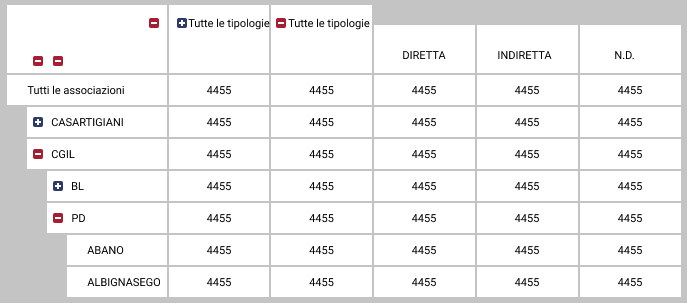
\includegraphics[scale=0.55]{./immagini/mockup-generale.png}
	}
\end{minipage}
\mbox{} 
\\
\\
Da questo mockup generale ho individuato i seguenti componenti grafici. In particolare ho definito la loro gerarchia di composizione:
\begin{itemize}
	\item \verb|Table|
	\begin{itemize}
		\item \verb|TableActionUI|
		\item \verb|TableHeader|
		\begin{itemize}
			\item \verb|TableLabel|
		\end{itemize}
		\item \verb|TableSidebar|
		\begin{itemize}
			\item \verb|TableLabel|
		\end{itemize}
		\item \verb|TableBody|
	\end{itemize}
\end{itemize}

\noindent
In seguito ho suddiviso il componente \verb|Table| in quattro quadranti utilizzando \verb|css grid|. Ogni quadrante conterrà i singoli componenti. \\
Per quanto riguarda \verb|TableActionUI| ho pensato di suddividerlo in quattro quadranti in modo similare a \verb|Table| così da posizionare i pulsanti delle azioni in modo semplice.
In \verb|TableBody| ho definito la sua struttura come una tabella html.
Nel componente \verb|TableHeader| ho deciso di realizzare una tabella per ogni dimensione disponibile con una singola riga contenente un'insieme di \verb|TableLabel|.
Il componente \verb|TableSidebar| è simile a \verb|TableHeader|, quindi per ogni dimensione disponibile viene creata una tabella con una singola colonna contenente un'insieme di \verb|TableLabel|.
Infine per quanto riguarda il componente \verb|TableLabel| ho pensato di realizzarlo con un elemento \verb|<th>| con al suo interno un possibile pulsante per l'azione eseguibile e una etichetta, posizionati mediante l'uso di \verb|css flex|.








%**************************************************************
%\section{Introduzione al progetto}

%**************************************************************
%\section{Analisi preventiva dei rischi}

%Durante la fase di analisi iniziale sono stati individuati alcuni possibili rischi a cui si potrà andare incontro.
%Si è quindi proceduto a elaborare delle possibili soluzioni per far fronte a tali rischi.\\

%\begin{risk}{Performance del simulatore hardware}
%    \riskdescription{le performance del simulatore hardware e la comunicazione con questo potrebbero risultare lenti o non abbastanza buoni da causare il fallimento dei test}
%    \risksolution{coinvolgimento del responsabile a capo del progetto relativo il simulatore hardware}
 %   \label{risk:hardware-simulator} 
%\end{risk}

%**************************************************************
%\section{Requisiti e obiettivi}


%**************************************************************
%\section{Pianificazione}